%option
\documentclass{standalone}
\usepackage{pgf-umlcd}
\renewcommand{\unidirectionalAssociation}[4]
{
  \draw[umlcd style, ->] (#1) -- (#4)
  node[near end, auto]{#2}
  node[near end, auto,swap]{#3};
}
\begin{document}
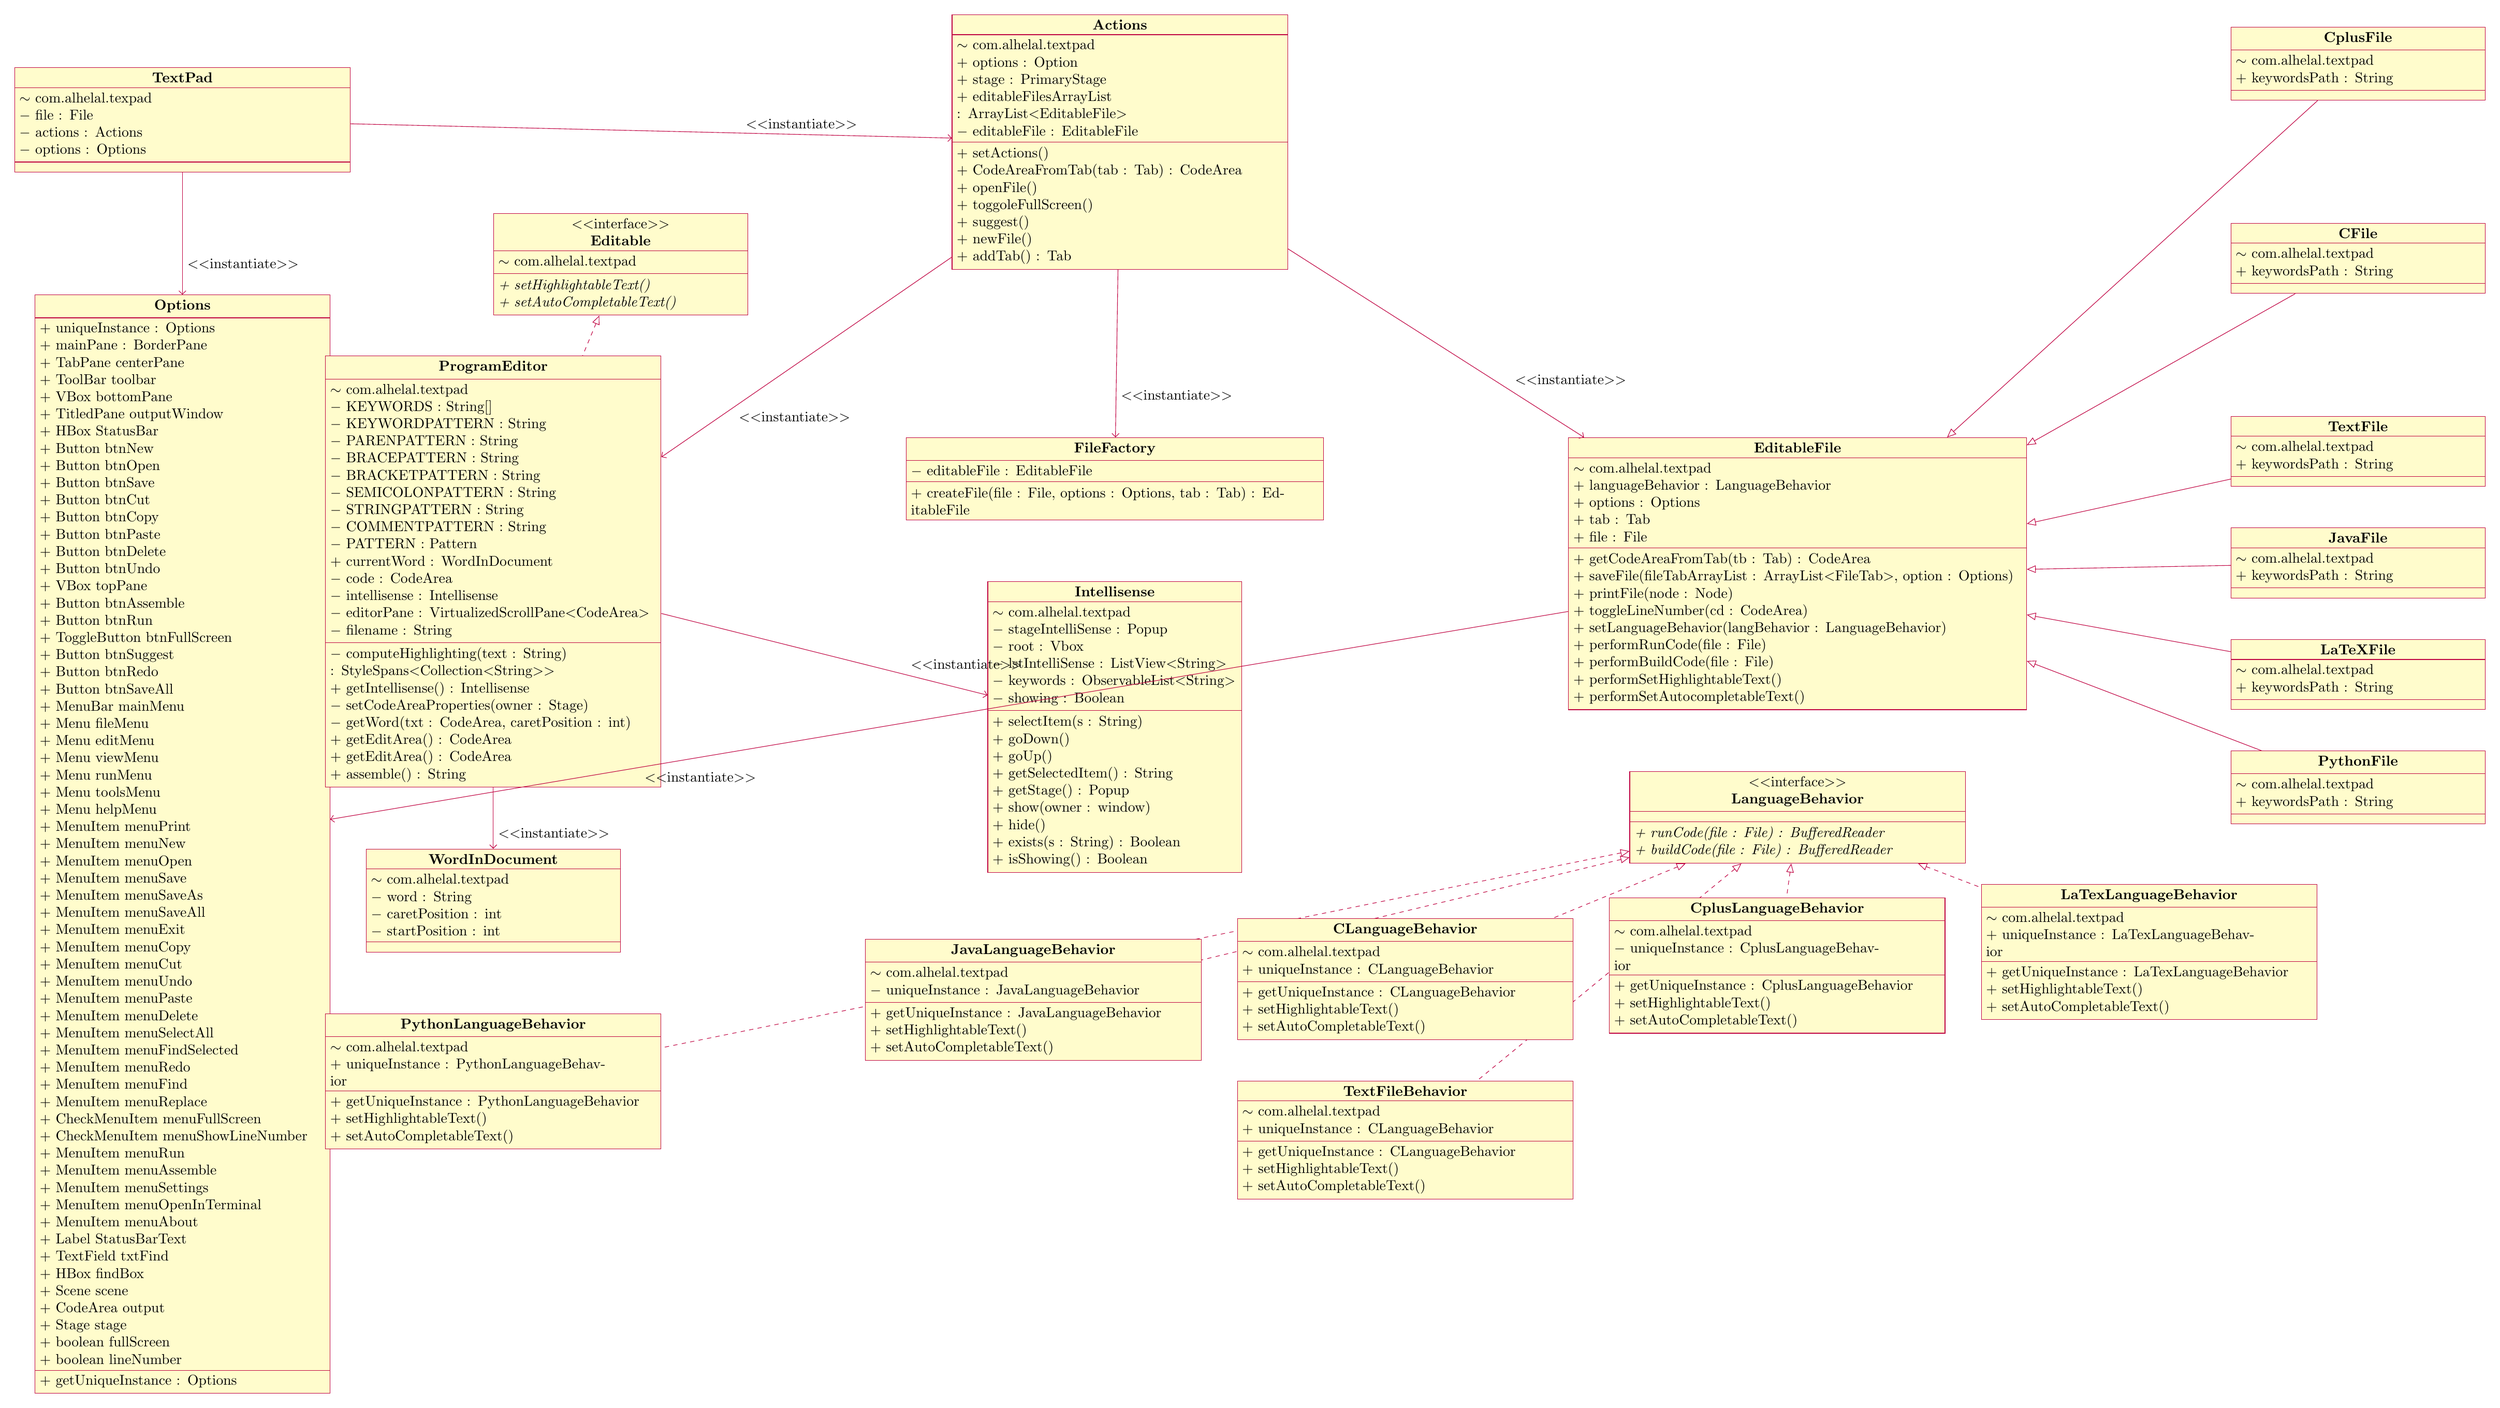
\begin{tikzpicture}
  \begin{class}[text width= 8cm]{TextPad}{0,0}
    \attribute{$\sim$ com.alhelal.texpad}
    \attribute{$-$ file : File}
    \attribute{$-$ actions : Actions}
    \attribute{$-$ options : Options}
  \end{class}

  \begin{class}[text width = 7cm,anchor=north,yshift=-3cm]{Options}{TextPad.south}
    \attribute{+ uniqueInstance : Options}
    \attribute{+ mainPane : BorderPane }
    \attribute{+ TabPane centerPane}
    \attribute{+ ToolBar toolbar}
    \attribute{+ VBox bottomPane}
    \attribute{+ TitledPane outputWindow}
    \attribute{+ HBox StatusBar}
    \attribute{+ Button btnNew}
    \attribute{+ Button btnOpen}
    \attribute{+ Button btnSave}
    \attribute{+ Button btnCut}
    \attribute{+ Button btnCopy}
    \attribute{+ Button btnPaste}
    \attribute{+ Button btnDelete}
    \attribute{+ Button btnUndo}
    \attribute{+ VBox topPane}
    \attribute{+ Button btnAssemble}
    \attribute{+ Button btnRun}
    \attribute{+ ToggleButton btnFullScreen}
    \attribute{+ Button btnSuggest}
    \attribute{+ Button btnRedo}
    \attribute{+ Button btnSaveAll}
    \attribute{+ MenuBar mainMenu}
    \attribute{+ Menu fileMenu}
    \attribute{+ Menu editMenu}
    \attribute{+ Menu viewMenu}
    \attribute{+ Menu runMenu}
    \attribute{+ Menu toolsMenu}
    \attribute{+ Menu helpMenu}
    \attribute{+ MenuItem menuPrint}
    \attribute{+ MenuItem menuNew}
    \attribute{+ MenuItem menuOpen}
    \attribute{+ MenuItem menuSave}
    \attribute{+ MenuItem menuSaveAs}
    \attribute{+ MenuItem menuSaveAll}
    \attribute{+ MenuItem menuExit}
    \attribute{+ MenuItem menuCopy}
    \attribute{+ MenuItem menuCut}
    \attribute{+ MenuItem menuUndo}
    \attribute{+ MenuItem menuPaste}
    \attribute{+ MenuItem menuDelete}
    \attribute{+ MenuItem menuSelectAll}
    \attribute{+ MenuItem menuFindSelected}
    \attribute{+ MenuItem menuRedo}
    \attribute{+ MenuItem menuFind}
    \attribute{+ MenuItem menuReplace}
    \attribute{+ CheckMenuItem menuFullScreen}
    \attribute{+ CheckMenuItem menuShowLineNumber}
    \attribute{+ MenuItem menuRun}
    \attribute{+ MenuItem menuAssemble}
    \attribute{+ MenuItem menuSettings}
    \attribute{+ MenuItem menuOpenInTerminal}
    \attribute{+ MenuItem menuAbout}
    \attribute{+ Label StatusBarText}
    \attribute{+ TextField txtFind}
    \attribute{+ HBox findBox}
    \attribute{+ Scene scene}
    \attribute{+ CodeArea output}
    \attribute{+ Stage stage}
    \attribute{+ boolean fullScreen}
    \attribute{+ boolean lineNumber}
    \operation{+ getUniqueInstance : Options}
  \end{class}

  \begin{interface}[text width=6cm,anchor=north west,xshift=4cm,yshift=2cm]{Editable}{Options.north east}
    \attribute{$\sim$ com.alhelal.textpad}
    \operation[0]{+ setHighlightableText()}
    \operation[0]{+ setAutoCompletableText()}
  \end{interface}
  
  \begin{class}[text width = 8cm,anchor=west,xshift=5cm,yshift=3cm]{Actions}{Editable.east}
    \attribute{$\sim$ com.alhelal.textpad}
    \attribute{+ options : Option}
    \attribute{+ stage : PrimaryStage}
    \attribute{+ editableFilesArrayList : ArrayList$<$EditableFile$>$}
    \attribute{$-$ editableFile : EditableFile}
    \operation{+ setActions()}
    \operation{+ CodeAreaFromTab(tab : Tab) : CodeArea}
    \operation{+ openFile()}
    \operation{+ toggoleFullScreen()}
    \operation{+ suggest()}
    \operation{+ newFile()}
    \operation{+ addTab() : Tab}
  \end{class}
%
  \begin{class}[text width = 8cm, yshift=-1.5cm,xshift=4cm]{ProgramEditor}{Options.north east}
    \implement{Editable}
    \attribute{$\sim$ com.alhelal.textpad}
    \attribute{$-$ KEYWORDS : String[]}
    \attribute{$-$ KEYWORDPATTERN : String}
    \attribute{$-$ PARENPATTERN : String}
    \attribute{$-$ BRACEPATTERN : String}
    \attribute{$-$ BRACKETPATTERN : String}
    \attribute{$-$ SEMICOLONPATTERN : String}
    \attribute{$-$ STRINGPATTERN : String}
    \attribute{$-$ COMMENTPATTERN : String}
    \attribute{$-$ PATTERN : Pattern}
    \attribute{+ currentWord : WordInDocument}
    \attribute{$-$ code : CodeArea}
    \attribute{$-$ intellisense : Intellisense}
    \attribute{$-$ editorPane : VirtualizedScrollPane$<$CodeArea$>$}
    \attribute{$-$ filename : String}
    \operation{$-$ computeHighlighting(text : String) : StyleSpans$<$Collection$<$String$>>$}
    \operation{+ getIntellisense() : Intellisense}
    \operation{$-$ setCodeAreaProperties(owner : Stage)}
    \operation{$-$ getWord(txt : CodeArea, caretPosition : int)}
    \operation{+ getEditArea() : CodeArea}
    \operation{+ getEditArea() : CodeArea}
    \operation{+ assemble() : String}
  \end{class}
%
  \begin{class}[text width=10cm,anchor=north west,xshift=6cm,yshift=-2cm]{FileFactory}{ProgramEditor.north east}
    \attribute{$-$ editableFile : EditableFile}
    \operation{+ createFile(file : File, options : Options, tab : Tab) : EditableFile}
  \end{class}

%%Filetab
%
%%Editor
%%
  \begin{class}[text width = 11cm,anchor=north west, xshift=6cm]{EditableFile}{FileFactory.north east}
    \attribute{$\sim$ com.alhelal.textpad}
    \attribute{+ languageBehavior : LanguageBehavior} 
    \attribute{+ options : Options} 
    \attribute{+ tab : Tab}
    \attribute{+ file : File}
    \operation{+ getCodeAreaFromTab(tb : Tab) : CodeArea} 
    \operation{+ saveFile(fileTabArrayList : ArrayList$<$FileTab$>$, option : Options)}
    \operation{+ printFile(node : Node)}
    \operation{+ toggleLineNumber(cd : CodeArea)}
    \operation{+ setLanguageBehavior(langBehavior : LanguageBehavior)}
    \operation{+ performRunCode(file : File)}
    \operation{+ performBuildCode(file : File)}
    \operation{+ performSetHighlightableText()}
    \operation{+ performSetAutocompletableText()}
  \end{class}
%%
  \begin{class}[text width = 6cm,anchor=west,xshift=5cm,yshift=3cm]{TextFile}{EditableFile.east}
    \inherit{EditableFile}
    \attribute{$\sim$ com.alhelal.textpad}
    \attribute{+ keywordsPath : String}
  \end{class}
%
  \begin{class}[text width = 6cm,anchor=south,yshift=3cm]{CFile}{TextFile.north}
    \inherit{EditableFile}
    \attribute{$\sim$ com.alhelal.textpad}
    \attribute{+ keywordsPath : String}
  \end{class}
%
  \begin{class}[text width = 6cm,anchor=south,yshift=3cm]{CplusFile}{CFile.north}
    \inherit{EditableFile}
    \attribute{$\sim$ com.alhelal.textpad}
    \attribute{+ keywordsPath : String}
  \end{class}
%
  \begin{class}[text width = 6cm,yshift=-1cm]{JavaFile}{TextFile.south}
    \inherit{EditableFile}
    \attribute{$\sim$ com.alhelal.textpad}
    \attribute{+ keywordsPath : String}
  \end{class}

  \begin{class}[text width = 6cm,yshift=-1cm]{LaTeXFile}{JavaFile.south}
    \inherit{EditableFile}
    \attribute{$\sim$ com.alhelal.textpad}
    \attribute{+ keywordsPath : String}
  \end{class}
%
  \begin{class}[text width = 6cm,yshift=-1cm]{PythonFile}{LaTeXFile.south}
    \inherit{EditableFile}
    \attribute{$\sim$ com.alhelal.textpad}
    \attribute{+ keywordsPath : String}
  \end{class}
%%JavaKeyword
% % \begin{interface}[text width = 6cm]{JavaKeyword}{0,0}
% %   \attribute{$\sim$ com.alhelal.textpad}
% %   \attribute{$-$ KEYWORDS : String[]}
% %   \attribute{$-$ KEYWORD_PATTERN : String}
% %   \attribute{$-$ PAREN_PATTERN : String}
% %   \attribute{$-$ BRACE_PATTERN : String}
% %   \attribute{$-$ BRACKET_PATTERN : String}
% %   \attribute{$-$ SEMICOLON_PATTERN : String}
% %   \attribute{$-$ STRING_PATTERN : String}
% %   \attribute{$-$ COMMENT_PATTERN : String}
% %   \attribute{$-$ PATTERN : Pattern}
% %   \operation{$-$ computeHighlighting(text : String) : StyleSpans<Collection<String>>}
% % \end{interface}
% % \node [above=3mm] at (current bounding box.north) {Singleton Pattern};
%
%%WordInDocument
%
  \begin{class}[text width = 6cm,yshift=-1.5cm]{WordInDocument}{ProgramEditor.south}
    \attribute{$\sim$ com.alhelal.textpad}
    \attribute{$-$ word : String}
    \attribute{$-$ caretPosition : int}
    \attribute{$-$ startPosition : int}
  \end{class}
%%intellisense
%
  \begin{class}[text width = 6cm,yshift=-1.5cm]{Intellisense}{FileFactory.south}
    \attribute{$\sim$ com.alhelal.textpad}
    \attribute{$-$ stageIntelliSense : Popup}
    \attribute{$-$ root : Vbox}
    \attribute{$-$ lstIntelliSense : ListView$<$String$>$}
    \attribute{$-$ keywords : ObservableList$<$String$>$}
    \attribute{$-$ showing : Boolean}
    \operation{+ selectItem(s : String)}
    \operation{+ goDown()}
    \operation{+ goUp()}
    \operation{+ getSelectedItem() : String}
    \operation{+ getStage() : Popup}
    \operation{+ show(owner : window)}
    \operation{+ hide()}
    \operation{+ exists(s : String) : Boolean}
    \operation{+ isShowing() : Boolean}
  \end{class}
%
  \begin{interface}[text width=8cm,yshift=-1.5cm]{LanguageBehavior}{EditableFile.south}
    \operation[0]{+ runCode(file : File) : BufferedReader}
    \operation[0]{+ buildCode(file : File) : BufferedReader}
  \end{interface}
%
  \begin{class}[text width = 8cm,yshift=-1.5cm]{PythonLanguageBehavior}{WordInDocument.south}
    \implement{LanguageBehavior}
    \attribute{$\sim$ com.alhelal.textpad}
    \attribute{+ uniqueInstance : PythonLanguageBehavior}
    \operation{+ getUniqueInstance : PythonLanguageBehavior}
    \operation{+ setHighlightableText()}
    \operation{+ setAutoCompletableText()}
  \end{class}
%
  \begin{class}[text width = 8cm,anchor=west,xshift=5cm,yshift=2cm]{JavaLanguageBehavior}{PythonLanguageBehavior.east}
    \implement{LanguageBehavior}
    \attribute{$\sim$ com.alhelal.textpad}
    \attribute{$-$ uniqueInstance : JavaLanguageBehavior}
    \operation{+ getUniqueInstance : JavaLanguageBehavior}
    \operation{+ setHighlightableText()}
    \operation{+ setAutoCompletableText()}
  \end{class}
%
  \begin{class}[text width = 8cm,xshift=5cm,yshift=2cm]{CLanguageBehavior}{JavaLanguageBehavior.east}
    \implement{LanguageBehavior}
    \attribute{$\sim$ com.alhelal.textpad}
    \attribute{+ uniqueInstance : CLanguageBehavior}
    \operation{+ getUniqueInstance : CLanguageBehavior}
    \operation{+ setHighlightableText()}
    \operation{+ setAutoCompletableText()}
  \end{class}

  \begin{class}[text width = 8cm,yshift=-1cm]{TextFileBehavior}{CLanguageBehavior.south}
    \implement{LanguageBehavior}
    \attribute{$\sim$ com.alhelal.textpad}
    \attribute{+ uniqueInstance : CLanguageBehavior}
    \operation{+ getUniqueInstance : CLanguageBehavior}
    \operation{+ setHighlightableText()}
    \operation{+ setAutoCompletableText()}
  \end{class}
%
  \begin{class}[text width = 8cm,yshift=2cm, xshift=5cm]{CplusLanguageBehavior}{CLanguageBehavior.east}
    \implement{LanguageBehavior}
    \attribute{$\sim$ com.alhelal.textpad}
    \attribute{$-$ uniqueInstance : CplusLanguageBehavior}
    \operation{+ getUniqueInstance : CplusLanguageBehavior}
    \operation{+ setHighlightableText()}
    \operation{+ setAutoCompletableText()}
  \end{class}
%
%
  \begin{class}[text width = 8cm,yshift=2cm,xshift=5cm]{LaTexLanguageBehavior}{CplusLanguageBehavior.east}
    \implement{LanguageBehavior}
    \attribute{$\sim$ com.alhelal.textpad}
    \attribute{+ uniqueInstance : LaTexLanguageBehavior}
    \operation{+ getUniqueInstance : LaTexLanguageBehavior}
    \operation{+ setHighlightableText()}
    \operation{+ setAutoCompletableText()}
  \end{class}
  \unidirectionalAssociation{Actions}{$<<$instantiate$>>$}{}{ProgramEditor}
  \unidirectionalAssociation{Actions}{$<<$instantiate$>>$}{}{FileFactory}
  \unidirectionalAssociation{Actions}{$<<$instantiate$>>$}{}{EditableFile}
  \unidirectionalAssociation{EditableFile}{$<<$instantiate$>>$}{}{Options}
  \unidirectionalAssociation{ProgramEditor}{$<<$instantiate$>>$}{}{WordInDocument}
  \unidirectionalAssociation{ProgramEditor}{$<<$instantiate$>>$}{}{Intellisense}
  \unidirectionalAssociation{TextPad}{$<<$instantiate$>>$}{}{Actions}
  \unidirectionalAssociation{TextPad}{$<<$instantiate$>>$}{}{Options}
\end{tikzpicture}
  \end{document}
